\documentclass[twoside,11pt]{article}

% Any additional packages needed should be included after jmlr2e.
% Note that jmlr2e.sty includes epsfig, amssymb, natbib and graphicx,
% and defines many common macros, such as 'proof' and 'example'.
%
% It also sets the bibliographystyle to plainnat; for more information on
% natbib citation styles, see the natbib documentation, a copy of which
% is archived at http://www.jmlr.org/format/natbib.pdf

\usepackage{jmlr2e}
\usepackage[ruled,vlined]{algorithm2e}

% Definitions of handy macros can go here

\newcommand{\dataset}{{\cal D}}
\newcommand{\fracpartial}[2]{\frac{\partial #1}{\partial  #2}}

% Heading arguments are {volume}{year}{pages}{date submitted}{date published}{paper id}{author-full-names}

%\jmlrheading{1}{2000}{1-48}{4/00}{10/00}{meila00a}{Marina Meil\u{a} and Michael I. Jordan}

% Short headings should be running head and authors last names

\ShortHeadings{Alternating Transfer Learning}{Fornia}
\firstpageno{1}

\begin{document}

%\title{Machine Learnable Image Compression Using Convolutional Autoencoders}
\title{Using Alternating Transfer Learning to Create Multi-Purpose Layers
in Deep Convolutional Neural Networks}

\author{\name R. Paul Fornia \email paulfornia@gmail.com \\
       \addr Department of Computer Science\\
       Johns Hopkins University\\
       Baltimore, MD, USA
       %\AND
       %\name bob...\\
       }

%\editor{Kevin Murphy and Bernhard Sch{\"o}lkopf}

\maketitle

\begin{abstract}%   <- trailing '%' for backward compatibility of .sty file
In transfer learning, image classification neuarl network layers can be initialized by 
parameters of a pre-trained neural network (e.g.,
an autoencoder (AE), or a Convolutional Neural Network (CNN) from a different
classification task).
But these layers are then fine-tuned to better 
fit the new task. In other words, transfer learning still produces a new, distinct
network.

I extend this idea by producing early layers of parameters that 
actually fit into
a high performing AE and a high performing CNN classifier simultaneously. 
This is the first neural network architecture I am aware of that has parameters shared between
multiple tasks.

First, I test the effectiveness of creating these layers simply from an AE or a CNN,
and then applying them in a fixed, non-trainable way to the opposite context
(AE trained on classification layers,
and vice-versa). This differs from transfer learning in that the layers are not
subsequently fine tuned.
Next, I propose a methodology called Alternating Transfer Learning (ATL)
that transfers the layers
back and forth between the two contexts.

Finally, I test the application of ATL to images from an entirely different domain.

Of these four methods, only (in-domain) ATL performs highly,
and nearly matches performance of the more traditional AE and CNN trained end-to-end.
The other three tests perform respectably, and may be sufficient for some appications,
but fall short of the performance of the traditional baselines.

I discuss potential applications, including
generating lossy compressed image representation on which inference can be
performed without the need to first decompress the image. Further refinement of 
the ideas proposed in this paper are needed before such applications are practical
or valuable.

%practical image compression framework that performs well as both 
%a) a traditional file compression and b) a feature set for which image 
%classification can be performed with high accuracy. If successful, this would 
%allow for highly accurate image classification to be applied directly to compressed 
%images and may speed up training and fitting of image classifiers. I 
%begin with a simplified version of the Compressive AE (CAE), 
%which has already demonstrated 
%promise as an image compression system, but which has not been tested directly 
%in classification. I also propose a \emph{context-specialized} image compression, in
%which an AE (such as a CAE) is used to initialize a classification problem, the 
%labels are used to fine-tune the Deep Convolutional Neural Network (DNN)
% (as has been discussed in the classification
%literature), a middle layer is quantized and taken as the compression, and new 
%layers are trained on the compression (using the original image as the output) 
%to turn it back into an effective AE.
\end{abstract}

\begin{keywords}
    Autoencoder, Compression, Convolutional Neural Network, Image Classification
\end{keywords}




\section{Background and Literature}

\subsection{Image Classification in Practice and Motivation}
The use of images in data pipelines is extremely common across industries and 
domains. Many of these applications include both image fil      e compression and 
image classification steps. But many modern pipelines approach these as two 
separate problems – often first ingesting and compressing
images for storage, and then when needed for classification 
(training or fitting), they must be uncompressed back into a lossy version, 
similar to their original human-readable form.

 For instance, Facebook has published details of both compression and their 
facial recognition algorithm, and there is no indication that the two systems 
are integrated \citep{collet2016zstandard, taigman2014deepface}.

\subsection{Existing Efforts}

As several authors have noted, 
there would be considerable value in being able to perform machine learning 
tasks directly on the compressed images. \citet{needell2017} has written a classification 
algorithm that can be performed on any general binary file structure (including 
state-of-the art image compression methods), but this approach has not yet shown
 competitive classification performance. 

Conversely, \citet{fu2016} showed strong 
classification performance, but on cosine distance, which is not a competitive 
compression algorithm. The same can be said for any approach that performs 
embeddings or feature extraction, which can be viewed as a form of compression 
designed specifically for one ML task.

I seek a balanced approach that perform as well at compression,
and for which the compressed images 
can be classified without the need for decompression, with out-of-sample
 classification accuracy near that of an analogous CNN trained end-to-end.

I begin with the AE, which was originally 
devised as a compression algorithm, and has also inspired many elements of 
deep learning, which is the backbone of virtually all competitive image 
classification algorithms today.
AEs have many practical applications outside of compression, including 
pretraining deep neural networks, feature extraction, 
and image de-noising \citep{baldi2012autoencoders}. While some authors have claimed that AEs do 
not have practical value as compression algorithms
\footnote{
Multiple practical guides make this claim. For instance, \citet{huben2018_tds_ae} states ``autoencoders will 
do a poor job for [out-of-sample] image compression... JPEG will do vastly better.''
}
, recent work by 
\citet{theis2017} proposes a compressive, convolution autoencoder (CAE) that 
has shown great promise as an effective, practical image compression method, 
competitive with the JPEG file format.

\subsection{Contributions}

This paper proposes a “balanced” image compression 
standard, namely, one that a) is competitive
to the AE as a compression technique, and b) can be used directly as a 
machine learning feature set in a way 
that provides competitive classification rates. Since AEs have already been explored 
at length as both compressors and as feature engineering methods, the first contribution 
of this paper is modest, and will simply “connect-the-dots” by finding one AE that 
works well at both tasks. 
To the best of my knowledge, this simple step does not appear in the literature as of early 2019.

Specifically, I will more thoroughly test the use of the AE’s bottleneck layer as a fixed feature set in image classification. This can also be interpreted as using the AE to “pretrain” a DNN, but with fixed weights in the ``left" half\footnote{I will refer to NNs as running left-to-right, moving from the input data to the labeled data} of the network, and not allowing these initial weights to be “fine-tuned”. 
This idea is not inherently novel, and has been shown to be effective \citep{bengio2006pretrain}, 
but has not been shown using an AE that simultaneously performs well as a compression algorithm. 
This is completely unsupervised, and does not rely on labels other than the image itself.

Next, I propose a supervised image compression. This version begins by training a 
classification CNN using labeled data, then fixes the initial layers and trains a 
new set of layers to convert it back into the original image, thus making an effective AE. 
In contrast to the CAE, this method has been widely studied as a classifier 
(and achieves state-of-the art accuracy), but has not been fully explored as a compression technique.

Finally, I will improve upon these ideas by allowing the early layers to be fine-tuned
little by little.
By moving the early layers back and forth between tasks, I find a set of early parameters
that compress the image, and perform well on both compression and classification tasks.
Since this is essentially just iterative, repetitive transfer learning between tasks,
I called this ``Alternating Transfer Learning''.





\section{Methodology} \label{fixed}

For all techniques proposed in this paper, the intended compression framework has
three high-level components to its architecture, which are
 illustrated in Figure \ref{fig:three_stages}:
\begin{enumerate}
    \item Compression layers, which is similar to the ``left half'' of either an AE or CNN. 
    \item Decompression layers, which is similar to the ``right half'' of an AE. 
    \item Classification layers, which can be interpreted as either the right half of
     an end-to-end CNN classifier, or as the entire classifier trained on extracted (compressed) features. This portion can easily and quickly be retrained for each new classification problem.
\end{enumerate}

All methodologies tried in this paper produce these three components.

\begin{figure}[h]
  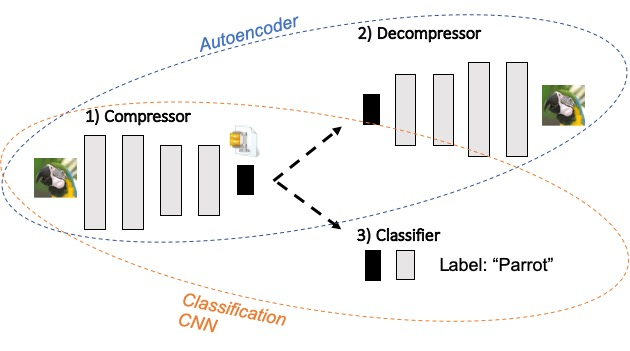
\includegraphics[width=\linewidth]{figures/three_stages.jpg}
  \caption{The three-stage machine learnable compression framework contains a compressor, a decompressor, and a classifier. Stages 1 and 2 together make an AE, stages 1 and 3 together make a DNN classifier. This paper considers the sharing of the compressor between both tasks. }
  \label{fig:three_stages}
\end{figure}

\subsection{Classification from AE-driven Compression} \label{general}

For the first methodology, I start with an AE approach in order 
to produce a traditional compression on the image data (components 1 and 2). 
I then take the resulting compressed data (i.e., the bottleneck layer) and attempt 
to perform classification on
the compressed data to predict the categorical labels (component 3).
This process is illustrated in Figure \ref{fig:general}.

\begin{figure}[h]
  \includegraphics[width=\linewidth]{figures/general.jpg}
  \caption{The AE-driven compression framework. Blue layers are trained as AEs. Green layers are trained as DNN classifiers.}
  \label{fig:general}
\end{figure}

I will test the hypothesis that this classifier will perform on compressed data 
nearly as well as state-of-the-art classifiers on full-sized images. 
As the compressors did not utilize the labels, this hypothesis could be tested on 
any labeling domain, such as facial recognition, object recognition, or digit classification.

\subsection{Decompression from Classifier-driven Compression} \label{special}

Having tested the efficacy of AE layers in a classifier, I similarly test using layers in an
AE that are constructed in a classification DNN.
I first replicate a high-performing DNN classifier from the literature. 
I then select one of the hidden layers, and apply 
quantization techniques similar to those described in \citet{hubara2018}. This hidden layer 
will act as the compressed image. This DNN will make up components 1 and 3. I 
will then use the original image to train a new decompression layer (component 2).  
This is illustrated in Figure \ref{fig:specialized}.

\begin{figure}[h]
  \includegraphics[width=\linewidth]{figures/specialized.jpg}
  \caption{The Classifier-driven compression framework.}
  \label{fig:specialized}
\end{figure}

Since components 1 and 2 are effectively built off standard DNN classifiers, 
this model’s efficacy as a classifier has already been shown at length in the 
literature \citep{krizhevsky2012imagenet}. I will reproduce this finding to create a 
baseline performance level. I then test whether 
the decompressor performs similarly to the analogous end-to-end AE.



\subsection{Alternating Transfer Learning} \label{alternate}

In section \ref{results} below, I will show that the performances of the above methods are limited. 
Simply copying the lower layers from one context to another 
does not provide performance comparable to end-to-end training. 
Thus, the compression obtained by an AE
is not an effective feature set for classification, and the lower levels of a classifier 
CNN do provide parameters for a competitive compression technique. This supports the conventional wisdom 
in the transfer learning literature than the early layers must be fine-tuned with the
labels of the new task.

Having shown that an AE or CNN alone does not produce a good general-purpose compression,
the question still remains on whether any such compression exists. 
The idea presented in this section is simple, and is motivated by 
the standard transfer learning procedure. In short, I continuously transfer the shared
initial layers back-and-forth between different contexts while training until results converge. 

The proposed technique is shown in Algorithm \ref{alg:alternate}.

\begin{algorithm}[H]
\SetAlgoLined
\KwResult{Compression, Decompression, and Classification NN components}
 Initialize model parameters for compression, decompression and classification layers;
 \While{Either Classifier or AE Performance is improving}{
  %\eIf{condition}{
  % instructions1\;
  % instructions2\;
  % }{
  % instructions3\;
  %}
  Train entire AE (compressor and decompressor) for $k_{AE}$ epochs\;

  Train only Classifier layers for $j$ epochs, as in Section \ref{fixed}\;

  Measure Classification performance\;

  Train entire Classification CNN (compressor and classifier) for $k_{Class}$ epochs\;

  Train only Decompressor layers for $j$ epochs\;

  Measure AE performance\;
 }
 Fine tune only Classifier layers by training a few epochs;

 Fine tune only Decompressor layers by training a few epochs;
 \caption{Alternating Transfer Learning procedure}
 \label{alg:alternate}
\end{algorithm}


\subsection{Extension of ATL training to other domains}

The ATL methodology is interesting and unique, but the application is not immediately obvious.
Perhaps there may applications where inference is applied to a compressed image. 
However, as the training must be done ahead of time with images with labels from the 
same classification task, practical value is still limited. Since inference only must
only be performed once per image, it would not be difficult to classify the image at time of 
compression and store the class along with the image.

Greater value would come from machine learnable compression layers if the layers could
be learned in advance of having a classification problem, and then quickly learned without
need for decompressing images. One final approach I test is taking parameters from the ATL 
procedure learned on one domain of images, and then attempted to learn both a classifier
and a decompressor on images from a brand-new domain. While all experiments use unseen images from a test
set, this approach takes it a step further and trains these tasks in a brand new domain,
using images unlike those seen in training. 

This architecture is shown in Figure \ref{fig:ext_atl}.

\begin{figure}[h]
  \includegraphics[width=\linewidth]{figures/ext_atl.jpg}
  \caption{The extension of the Alternating Transfer Learning framework to a new domain.}
  \label{fig:ext_atl}
\end{figure}

As I discuss in the results section, this technique does not work well, and tasks from 
one domain are not able to be easily learned from the compressed layers that had been trained
using ATL on a different domain. 










\section{Experiments and Results} \label{results}


\subsection{Datasets}

I use three datasets in this paper:

\begin{enumerate}
\item{MNIST: Handwritten digits 0-9}
\item{KMNIST: Examples of ten handwritten Korean characters}
\item{Fashion-MNIST: Images of ten categories of clothing or accessories}
\end{enumerate}

These datasets are all greyscale, all 28x28 pixels, and all consist of ten classes.
In fact, KMNIST and Fashion-MNIST were created as easy ``drop-in'' replacements for MNIST.
A future direction of research could be to test color images and images of varying sizes.
Using images from different domains can provide a starting point for transferring 
compression representations, even if the structure of the images from the different 
domains is very similar.

\subsection{Performance Metrics}

As all three datasets contain ten well-balanced classes, I simply use accuracy to measure
effectiveness of classification. 

\begin{equation}
Accuracy = \frac{Correct\ Predictions}{Total\ Predictions}
\end{equation}

For the AE, I measure performance by Peak Signal to Noise Ratio (PSNR), 
a conversion of Mean Squared Error (MSE) into the decibel scale, which is a common
performance metric of reconstructing lossy image compressions.

\begin{equation}
PSNR = 10*log_{10}\left(\frac{MAX^2_I}{MSE}\right)
\end{equation}

Where $MAX_I$ is the maximum pixel value, e.g. 255.


\subsection{Architecture}

For this paper, I propose an architecture for experimental purposes.
There is one primary constraint on the architecture design as shown in Figure \ref{fig:three_stages}:
the initial layers of the AE must match initial layers of the classification network.
Here, ``initial layers of the AE'' mean all layers from the input to the bottleneck layer (inclusive).

I do not claim that the proposed architecture is the optimal one for this problem,
however, the architecture is loosely based on existing well performing networks, and so 
results are still strong enough for many practical applications.
Future research could focus on improvements to this architecture.

I begin with the well-known but simple LeNet-5 architecture %\cite{}
, with a small modification to account for the size of the MNIST data.
I also add dropout layers in the fully connected portion of the graph. 
This powerful addition helps prevent overfitting, and was popularized long
after the publication of LeNet-5. %\cite{}

The LeNet architecture also has another valuable property: a good bottleneck layer.
The last convolutional layer of LeNet contains about half the parameters of the input,
similar to many AE architectures. 

To create the Decompression layers, I simply work backwards from the compression layers of LeNet,
using similar convolutions, and upsample layers in place of maxpool layers.

Finally, I add a quantization to the bottleneck layer by rounding output values. %\cite{}
The input values of the datasets contain 28x28 pixels of integer values between 1 and 255.
The uncompressed image therefore can be represented by $28*28*log2(256) = 6272 = 784$ bytes.
The bottleneck layers contains 16 5x5 filters. 
After rounding the compressed values, outputs were integers between 0 and 15,
allowing compressed images to be stored in just $16*5*5*log2(16) = 1600 = 200$ bytes,
for a data compression ratio of 3.9, or space savings of 74.5\%. 

%%Table of architecture here%%

\begin{table}[h]
  \centering
  \begin{tabular}{|c|c||c|c||c|c|}
    \hline
    %\multicolumn{2}{|c|}{Baseline (50 Epochs of Training)}\\
    %\hline
    \multicolumn{2}{|c||}{1) Compressor} & 
    \multicolumn{2}{|c||}{2) Decompressor} & 
    \multicolumn{2}{|c|}{3) Classifier}\\  
    \hline
    Layer Type & Output & Layer Type & Output & Layer Type & Output \\  
    \hline
    Input & 1x28x28 & Compressed Input & 16x5x5 & Compressed Input & 16x5x5\\  
    \hline
    6 5x5 Conv Filters & 6x24x24 & Upscale & 16x10x10 & Flatten & 400\\  
    \hline
    Padding & 6x28x28 & Padding & 16x14x14 & Full Layer & 120\\  
    \hline
    Max Pooling 2x2 & 6x14x14 & 16 3x3 Convolutions & 16x12x12 & 50\% Dropout & 120\\  
    \hline
    16 5x5 Conv Filters & 16x10x10 & Upscale & 16x24x24 & Full Layer & 84\\  
    \hline
    Max Pooling 2x2 & 16x5x5 & Padding & 16x28x28 & 50\% Dropout & 84\\  
    \hline
     &  & 6 3x3 Convolutions & 6x26x26 & Full Layer & 10\\  
    \hline
     &  & Padding & 6x30x30 &  & \\  
    \hline
     &  & 1 3x3 Convolution & 1x28x28 &  & \\  
    \hline

  \end{tabular}
  \caption{The architecture used for these experiments, broken into the three components
    described in Section \ref{fixed}}
  \label{table:base}
\end{table}



\subsection{Baseline AE and Classifier}

While the architecture above is based on a classifier with good performance,
the architecture (especially the AE) is not necessarily state-of-the art. 
So in order to measure performance, I first run 50 epochs of both the full AE and Classifier,
both with randomly initialized parameters, allowing for the full network to be trained,
just as a traditional DNN would be. I measure performance on the test dataset as training progresses,
and find that improvement has leveled off by the 50th epoch.
This provides a good best-case-scenario benchmark for performance of the AE and Classifier. 

%%%Table of Baseline findings%%%%
%\begin{table}
%  \centering
%  \includegraphics[]{figures/table_baseline.jpg}
%  \caption{Baseline performance metrics of the full AE and Classification CNN. 
%   Measured on an out-of-sample test dataset after 50 epochs of training.}
%  \label{table:base}
%\end{table}

\begin{table}[h]
  \centering
  \begin{tabular}{|c||c|c|}
    \hline
    \multicolumn{3}{|c|}{Baseline (50 Epochs of Training)}\\
    \hline
    Dataset & Classification Accuracy & Decompression PSNR \\
    \hline
    MNIST & 98.6\% & 22.8\\
    \hline
    KMNIST & 89.9\% & 17.0\\
    \hline
    Fashion & 85.7\% & 18.2\\
    \hline
  \end{tabular}
  \caption{Baseline performance metrics of the full AE and Classification CNN. 
   Measured on an out-of-sample test dataset after 50 epochs of training.}
  \label{table:base}
\end{table}

\subsection{AE-Driven Compression Experiment}

As described in section \ref{general}, I start with the baseline AE.
Using the lower layers, I compress all the images. This in effect ``freezes'' the 
lower layer parameters, and does not allow them to be fine tuned. 
I then train only the classifier layers on the compressed image.

%%%Insert Findings here%%%

\begin{table}[h]
  \centering
  \begin{tabular}{|c||c|c|}
    \hline
    \multicolumn{3}{|c|}{Classification trained on AE-Driven compression}\\
    \hline
    Dataset & Baseline Accuracy & Accuracy on Compressed Data \\
    \hline
    MNIST & 98.6\% & 91.7\%\\
    \hline
    KMNIST & 89.9\% & 70.7\%\\
    \hline
    Fashion & 85.7\% & 79.8\%\\
    \hline
  \end{tabular}
  \caption{Performance metrics of the General Compression: 
   Accuracy on an out-of-sample test dataset after 50 epochs of training a classifier on
   data compressed by the AE.}
  \label{table:general}
\end{table}

I find that for all three datasets, the classification accuracy on the compressed images
is reasonably high (possibly good enough for some applications), but significantly 
short of the baseline.


\subsection{Classifier-Driven Compression Experiment}

As described in section \ref{special}, I start with the CNN that is trained by classification.
As above, I use the lower layers of this network to compress the image, then I train
only the decompressor layers on the compressed images, with the original images
as the target values.

%%Insert table%%

\begin{table}[h]
  \centering
  \begin{tabular}{|c||c|c|}
    \hline
    \multicolumn{3}{|c|}{AE trained on Classifier-Driven compression}\\
    \hline
    Dataset & Baseline PSNR & PSNR on Compressed Data \\
    \hline
    MNIST & 21.8 & 19.9\\
    \hline
    KMNIST & 17.0 & 15.4\\
    \hline
    Fashion & 18.2 & 17.8\\
    \hline
  \end{tabular}
  \caption{Performance metrics of the Specialized Compression: 
   PSNR on an out-of-sample test dataset after 50 epochs of training an AE on
   data compressed by the Classification CNN.}
  \label{table:special}
\end{table}

Just as with the classification based on the AE-driven compression attempt, 
I find an AE with some value, but with 
significantly worse performance than the AE that is trained from the original images.

\subsection{Alternating Transfer Learning Experiment}

Next, I test the idea described in Section \ref{alternate} by implementing Algorithm \ref{alg:alternate}.
For each of the three datasets seperately, I train the AE layers, then the Classification layers
(which include shared layers with the AE, which have now been initialized), then train the AE again,
and so on. I define an ``epoch set'' as one round of all four types of training as described in 
Algorithm \ref{alg:alternate}. For this experiment, I set $k_AE = k_class = j_AE = j_class = 1$, 
meaning each epoch set contains a total of four epochs (each of differing levels of complexity).
Further research is needed to optimized these hyperparameters.

For all three datasets, I perform 25 epoch sets. With a total of 100 epochs, this is roughly
similar run time to the above experiments, which require 50 full epochs (e.g., end-to-end AE
to train the network from scratch), and 50 epochs on the smaller network component 
(e.g., classification on the fixed, compressed image set).

%%%% Insert Findings %%%%

\begin{table}[h]
  \centering
  \begin{tabular}{|c||c|c|c|c|}
    \hline
    \multicolumn{5}{|c|}{Alternating Transfer Learning}\\
    \hline
    Dataset & Baseline PSNR  & PSNR from ATL & Baseline Accuracy & Accuracy from ATL \\   \hline
    MNIST & 21.8 & 22.8 & 98.6\% & 97.2\% \\   \hline
    KMNIST & 17.0 & 17.6 & 89.9\% & 85.5\% \\   \hline
    Fashion & 18.1 & 18.5 & 85.6\% & 85.2\% \\   \hline  

  \end{tabular}
  \caption{Performance metrics of the Alternating Transfer Learning:
   PSNR on an out-of-sample test dataset after 50 epochs of training an AE on
   data compressed by the Classification CNN.}
  \label{table:alternate}
\end{table}

As shown in table \ref{table:alternate}, this method outperforms the other methods proposed so far.
For all six tests (classification and AE for three datasets), the Alternating Transfer Learning 
approach significantly outperforms the simple fixed transfers described above. 

Classification accuracy of these approaches is slightly below that of the traditional 
end-to-end CNN approach, however, PSNR on the decompressed images actually exceeds that
of the traditional full AE, and performance rates over the epoch sets suggests further room
for improvement. 

\subsection{Extension to Other Domain}






\section{Discussion}

\subsection{Practical Implications}

To my knowledge, this paper is the first to provide a framework for training two 
seperate neural network architectures that share sets of parameters. 
While this is an interesting academic accomplishment, the networks that I trained 
in this paper via the ATL methodology fall short of having obvious practical applications.

The original motivation for this work was to find a compression method that could act as
the input to a classification CNN. If one considers the two tasks in classification,
training and inference, I succeeded at this goal in one sense and fell short in another. 
The ATL is a functioning compression algorithm for which inference can be performed directly
on the compressed version of the images, at greatly reduced speed. However, since labels
were used in creating the ATL, the training step itself was not performed on the compressed 
images, but rather on a combination of compressed and uncompressed images. 

This is unfortunate, since the practical implications for training on compressed images 
is more obvious than the implications for inference on compressed images. Training on 
compressed images would allow new widely applicable, general compression techniques to 
be used for general purpose image storage, with the knowledge that new problems could be
applied at a later time with decompressing. By contrast, in the classification task is
already known at the time the compression is developed (which it must be for ATL), 
then it is easy enough to simply perform inference at the time of
image compression, since the class label itself is trivially small to store. 

There is one possible scenario in which findings of this paper could have a direct, practical
application: those in which
fast training is more important than accuracy. In this case, the AE-driven compression
method can be used, and a classifier can be trained directly on the compressed image very quickly.
The results here show that this method gets an accuracy lower than a traditional 
classification CNN, but still far above random, and likely high enough for some applications.

\subsection{Run-Time}

\subsection{PyTorch Implementation}

I attempted versions of this project both in Tensorflow (via python) and PyTorch, 
and settled on PyTorch.
The methods in this paper have two unique implementation elements.
This first is to have an architecture
with two targets, two loss functions, etc.. Surprisingly, this was easy in both tools, by
simply having code for components 2) and 3) both reference the last layer from component 1).
Then, with some care, you can train 2) (which backpropagates to component 1)) without 
affecting component 3), and then train 3) without affecting 2).

The slightly trickier aspect was ``freezing'' the parameters in 1) altogether, 
which is a critical step for this approach, and which differentiates this from traditional
transfer learning. This can be done manually in any tool by simply performing inference
to get the outputs of the bottle-neck layer, then feeding this into a brand new NN as input,
and finally transfering the parameters back into the original architecture.

However, with PyTorch, this can be done simply with the detach() function.
This effectively freezes the value, and breaks the mapping of the backpropagation gradient, 
and preserves all prior layer parameters.

\subsection{Next Steps}

There are at least three obvious paths forward for future research, probably in the following order.

First, the ideas of ATL must be expanded to more practical training methodologies. 
More experimentation should be done to find other architectures with shared layers.
Using the three components proposed here, there are many possible 
ways to train this architecture, even if the architecture's components themselves are fixed.
One potential next step is to expand ATL beyond two domains. ATL accomplishes two tasks:
AE and Classification for one domain. But this could be easily expanded to more than one domain. 
Just from the data used in this study, ATL could be performed alternating between six different 
tasks: Decompressing MNIST, Classifying MNIST, Decompressing KMNIST, etc..
As it was performed in this paper, ATL trained on one domain did not extend to another.
But I would hypothesize that ATL trained on several domains may generalize to new ones better.  

Second, steps should be taken to be used on more realistic images. The methods described
in this paper could easy be extended to color images. Also, techniques could be explored that
are intended to handle images of differing sizes. A simple solution to this is rescaling,
but some architectures have been designed to handle different sized images
without the need for resizing. %\cite{squeezenet paper}
This would support the idea in the above paragraph, since handling images of differing sizes
would greatly increase the number of label classification sets available.


Finally, ideas should be incorporated from the AE literature to improve PSNR and the 
data compression rate. 
As a proof of concept, I used an AE that fit nicely with the classification network.
But state-of-the-art compressive AEs can achieve much higher PSNR with better data
compression ratios. For example, \citet{theis2017} achieves a PSNR of over 40 with 
substantially better compression ratios than what I use here. 
One challenge will be to find early layer architectures that balance the benefits
of both state-of-the-art
AEs, and state-of-the-art classifiers.  



%  blah blah sample citation ~\citep{pearl:88}.  Whether in their guise as 
%random fields), \emph{probabilistic graphical models} have a number 
%of uncertainty...\\

%{\noindent \em Remainder omitted in this sample. See http://www.jmlr.org/papers/ for full paper.}

% Acknowledgements should go at the end, before appendices and references

%\acks{We would like to acknowledge support for this project
%from the National Science Foundation (NSF grant IIS-9988642)
%and the Multidisciplinary Research Program of the Department
%of Defense (MURI N00014-00-1-0637). }

% Manual newpage inserted to improve layout of sample file - not
% needed in general before appendices/bibliography.

%\newpage

%\appendix
%\section*{Appendix A.}
%\label{app:theorem}

% Note: in this sample, the section number is hard-coded in. Following
% proper LaTeX conventions, it should properly be coded as a reference:

%In this appendix we prove the following theorem from
%Section~\ref{sec:textree-generalization}:

%\noindent
%{\bf Theorem} {\it Let $u,v,w$ be discrete variables such that $v, w$ do
%not co-occur with $u$ (i.e., $u\neq0\;\Rightarrow \;v=w=0$ in a given
%dataset $\dataset$). Let $N_{v0},N_{w0}$ be the number of data points for
%which $v=0, w=0$ respectively, and let $I_{uv},I_{uw}$ be the
%respective empirical mutual information values based on the sample
%$\dataset$. Then
%\[
%	N_{v0} \;>\; N_{w0}\;\;\Rightarrow\;\;I_{uv} \;\leq\;I_{uw}
%\]
%with equality only if $u$ is identically 0.} \hfill\BlackBox

%\noindent
%{\bf Proof}. We use the notation:
%\[
%P_v(i) \;=\;\frac{N_v^i}{N},\;\;\;i \neq 0;\;\;\;
%P_{v0}\;\equiv\;P_v(0)\; = \;1 - \sum_{i\neq 0}P_v(i).
%\]
%These values represent the (empirical) probabilities of $v$
%taking value $i\neq 0$ and 0 respectively.  Entropies will be denoted
%by $H$. We aim to show that $\fracpartial{I_{uv}}{P_{v0}} < 0$....\\

{%\noindent \em Remainder omitted in this sample. See http://www.jmlr.org/papers/ for full paper.}


\vskip 0.2in
%\bibliographystyle{unsrt}
\bibliography{paper}

\end{document}
